
\documentclass{beamer}
\usetheme{Electromagnetism}
\usepackage{Electromagnetism}
\graphicspath{{pictures/}}
% -------------------------------------- Grid
%-------------------------------------------------------
\makeatletter
\def\grd@save@target#1{%
  \def\grd@target{#1}}
\def\grd@save@start#1{%
  \def\grd@start{#1}}
\tikzset{
  grid with coordinates/.style={
    to path={%
      \pgfextra{%
        \edef\grd@@target{(\tikztotarget)}%
        \tikz@scan@one@point\grd@save@target\grd@@target\relax
        \edef\grd@@start{(\tikztostart)}%
        \tikz@scan@one@point\grd@save@start\grd@@start\relax
        \draw[minor help lines] (\tikztostart) grid (\tikztotarget);
        \draw[major help lines] (\tikztostart) grid (\tikztotarget);
        \grd@start
        \pgfmathsetmacro{\grd@xa}{\the\pgf@x/1cm}
        \pgfmathsetmacro{\grd@ya}{\the\pgf@y/1cm}
        \grd@target
        \pgfmathsetmacro{\grd@xb}{\the\pgf@x/1cm}
        \pgfmathsetmacro{\grd@yb}{\the\pgf@y/1cm}
        \pgfmathsetmacro{\grd@xc}{\grd@xa + \pgfkeysvalueof{/tikz/grid with coordinates/major step}}
        \pgfmathsetmacro{\grd@yc}{\grd@ya + \pgfkeysvalueof{/tikz/grid with coordinates/major step}}
        \foreach \x in {\grd@xa,\grd@xc,...,\grd@xb}
        \node[anchor=north] at (\x,\grd@ya) {\pgfmathprintnumber{\x}};
        \foreach \y in {\grd@ya,\grd@yc,...,\grd@yb}
        \node[anchor=east] at (\grd@xa,\y) {\pgfmathprintnumber{\y}};
      }
    }
  },
  minor help lines/.style={
    help lines,
    step=\pgfkeysvalueof{/tikz/grid with coordinates/minor step}
  },
  major help lines/.style={
    help lines,
    line width= 0.5pt,
    step=\pgfkeysvalueof{/tikz/grid with coordinates/major step}
  },
  grid with coordinates/.cd,
  minor step/.initial=.2,
  major step/.initial=1,
  major line width/.initial=2pt,
}
\makeatother
\usepackage{cancel}
\usetikzlibrary{shapes.geometric,calc}

\begin{document}


% ============================== Слайд ## ===================================
\begin{frame}{}{}
	\begin{center}
		\begin{tikzpicture}[>=latex, scale=1.2, transform shape]
			%                \node[anchor = center] at (0,0) {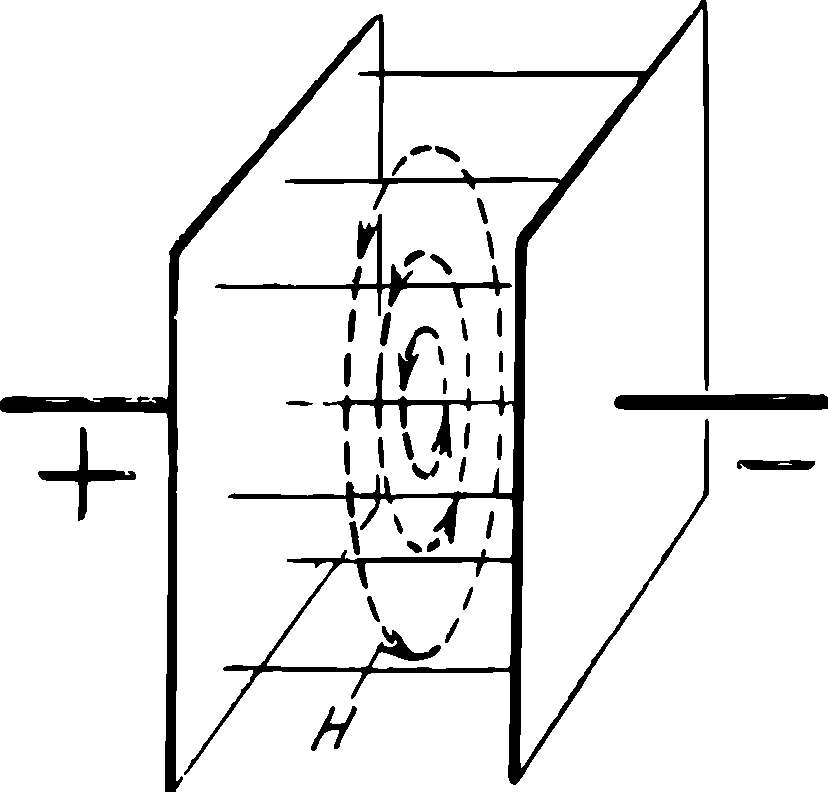
\includegraphics[width=2cm]{Pictures/condensator}};
			\draw[thick, red] (-1.5, 0) --  (-0.6, 0) node[pos=0.1, below] {$+$};
			\draw[fill=red!50] (-0.6, -1) -- (-0.6, 0.4) -- (-0.1, 0.9) -- (-0.1, -0.5) -- cycle;


			\foreach \x in {-1, 0, +1} {
					\begin{scope}[xshift=\x cm]
						\draw[blue, arrowpos={0.4}{2pt}{2pt}] (0,0) circle (0.2 and 0.6);
						\draw[blue, arrowpos={0.4}{2pt}{2pt}] (0,0) circle (0.14 and 0.4);
						\draw[blue, arrowpos={0.4}{2pt}{2pt}] (0,0) circle (0.05 and 0.2);
					\end{scope}

				}

			\draw[thick, red] (-1, 0) --  (-0.6, 0) ;


			\foreach \y in {0, -0.5, -1} {
					\begin{scope}[yshift=\y cm]
						\draw[arrowpos={0.4}{2pt}{2pt}, red, thin] (-0.2, 0.6) -- ++(0.8,0);
						\draw[arrowpos={0.4}{2pt}{2pt}, red, thin] (-0.3, 0.5) -- ++(0.8,0);
						\draw[arrowpos={0.4}{2pt}{2pt}, red, thin] (-0.4, 0.4) -- ++(0.8,0);
					\end{scope}
				}

			\begin{scope}[xshift=0.83cm]
				\draw[fill=blue!50] (-0.6, -1) -- (-0.6, 0.4) -- (-0.1, 0.9) -- (-0.1, -0.5) -- cycle;
			\end{scope}
			\draw[thick, blue] (0.5, 0) --  (1.5, 0) node[pos=0.9, below] {$-$};

			\draw[->] (-1.4, -1.2) -- node[below] {$I$} ++(0.6, 0);
			\draw[->] (-0.4, -1.2) -- node[below] {$\parttime\Dfield$} ++(0.6, 0);
			\draw[->] (1, -1.2) -- node[below] {$I$} ++(0.6, 0);

			\begin{scope}[xshift=4cm]
				%                \node[anchor = center] at (0,0) {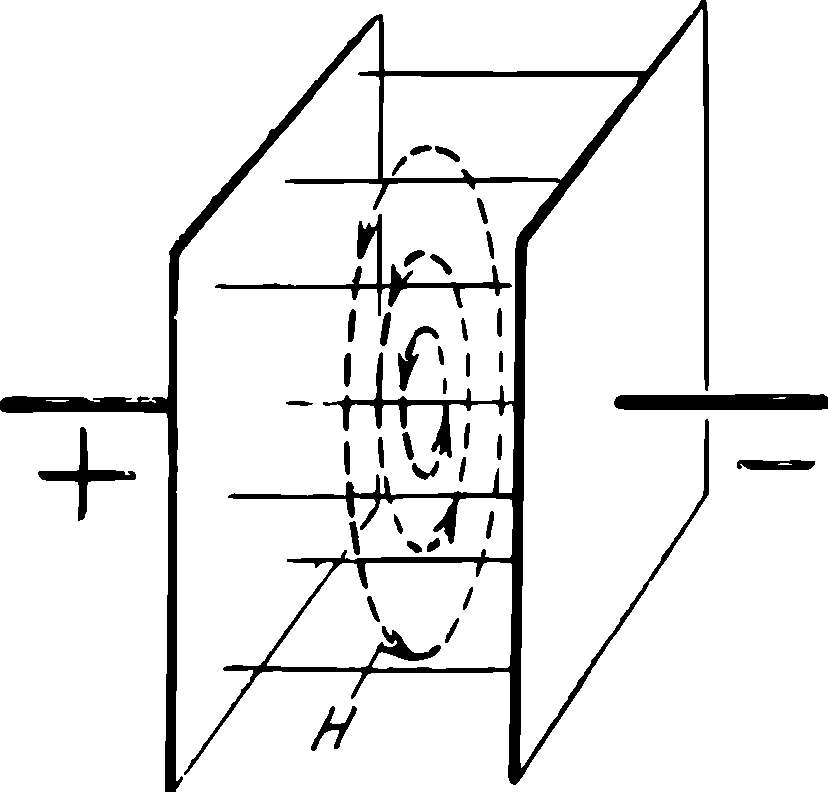
\includegraphics[width=2cm]{Pictures/condensator}};
				\draw[thick, red] (-1.5, 0) --  (-0.6, 0) node[pos=0.1, below] {$+$};
				\draw[fill=red!50] (-0.6, -1) -- (-0.6, 0.4) -- (-0.1, 0.9) -- (-0.1, -0.5) -- cycle;


				\foreach \x in {-1, 0, +1} {
						\begin{scope}[xshift=\x cm, xscale=-1]
							\draw[blue, arrowpos={0.4}{2pt}{2pt}] (0,0) circle (0.2 and 0.6);
							\draw[blue, arrowpos={0.4}{2pt}{2pt}] (0,0) circle (0.14 and 0.4);
							\draw[blue, arrowpos={0.4}{2pt}{2pt}] (0,0) circle (0.05 and 0.2);
						\end{scope}

					}

				\draw[thick, red] (-1, 0) --  (-0.6, 0) ;


				\foreach \y in {0, -0.5, -1} {
						\begin{scope}[yshift=\y cm]
							\draw[arrowpos={0.4}{2pt}{2pt}, red, thin] (-0.2, 0.6) -- ++(0.8,0);
							\draw[arrowpos={0.4}{2pt}{2pt}, red, thin] (-0.3, 0.5) -- ++(0.8,0);
							\draw[arrowpos={0.4}{2pt}{2pt}, red, thin] (-0.4, 0.4) -- ++(0.8,0);
						\end{scope}
					}

				\begin{scope}[xshift=0.83cm]
					\draw[fill=blue!50] (-0.6, -1) -- (-0.6, 0.4) -- (-0.1, 0.9) -- (-0.1, -0.5) -- cycle;
				\end{scope}
				\draw[thick, blue] (0.5, 0) --  (1.5, 0) node[pos=0.9, below] {$-$};

				\draw[<-] (-1.4, -1.2) -- node[below] {$I$} ++(0.6, 0);
				\draw[<-] (-0.4, -1.2) -- node[below] {$\parttime\Dfield$} ++(0.6, 0);
				\draw[<-] (1, -1.2) -- node[below] {$I$} ++(0.6, 0);
			\end{scope}
			%
			%                \draw (-2, -2) to[grid with coordinates] (3,3);
		\end{tikzpicture}
	\end{center}
\end{frame}
% ===========================================================================



\end{document}